\chapter{Appendix}

\section{Influence of $k$ on sensitivity to perturbations of $k$-NN graphs}

\begin{figure}[h]
  \centering
  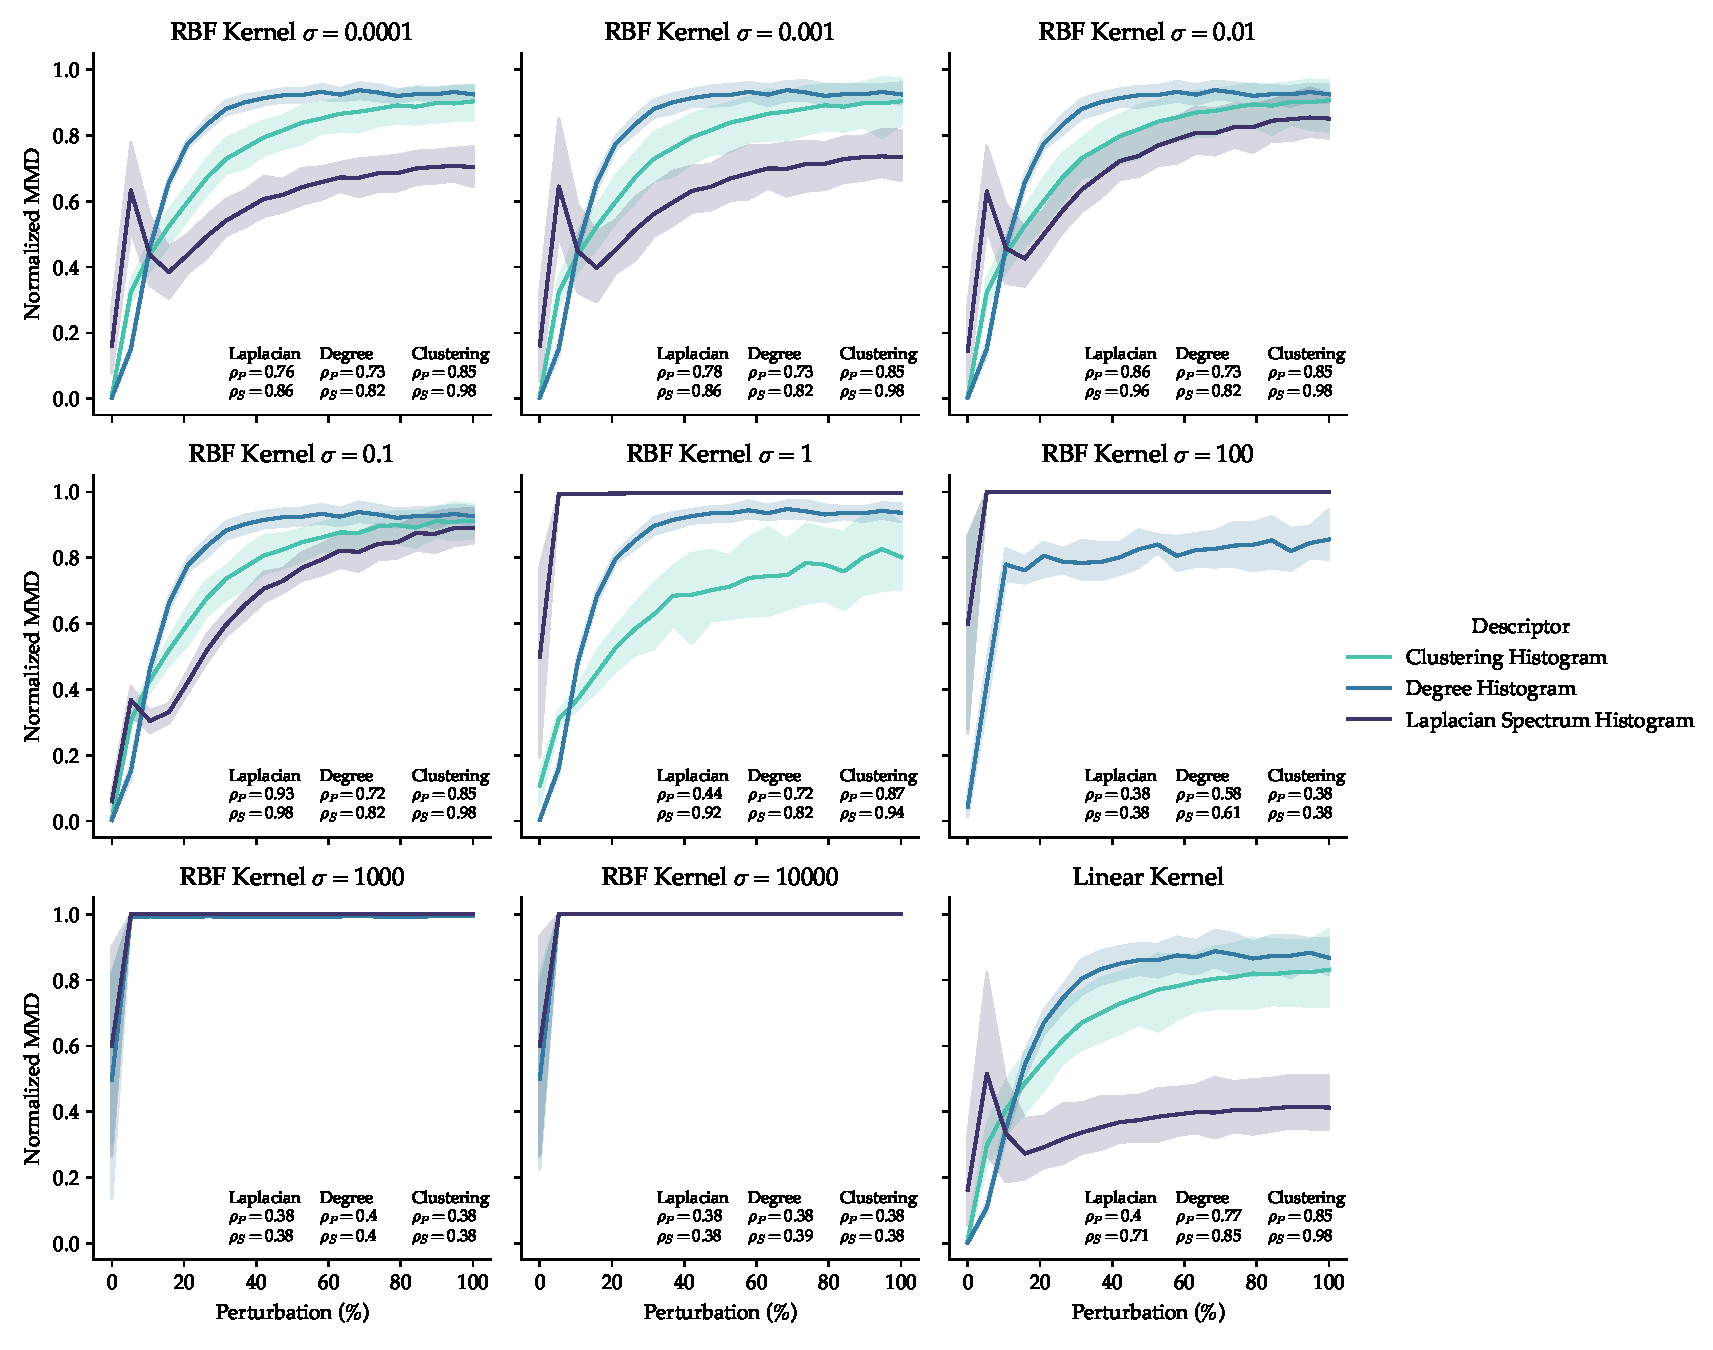
\includegraphics[width=\textwidth]{./figures/results/res_1_5.pdf}
  \caption[MMD vs. Gaussian Noise Perturbation (in \%) for various graph
descriptors of the 2-NN-graphs.]{MMD vs. Gaussian Noise Perturbation (in \%) for
various graph descriptors of the 2-NN-graphs. The kernel here is shown on top of
each subplots.}
  \label{fig:mmd_effect_kernel_knn}
\end{figure}


\section{Weisfeiler-Lehman Runtime Improvements for Sparse
  Graphs}\label{sec:sparse_wl}

In this thesis, we devised a three-pronged method to speed up the runtime of the
Weisfeiler-Lehman kernel by approximately 80\% by leveraging the sparsity of the
graphs used here. The three elements contributing to the speedup are the
following:

\begin{enumerate}
\item Our implementation parallelizes the execution of Weisfeiler-Lehman hash
computations since each graph's hash can be computed independently prior to
computing the kernel.
\item It also parallelizes the computation of similarity of graphs in RKHS by
computing batches of the inner products independently.
\item When comparing graphs, lots of CPU cycles are spent processing
positions/hashes that do not actually overlap between Weisfeiler-Lehman
histograms. As such, we manually loop over the overlapping keys, outperforming
numpy dot product-based implementations on collections of sparse graphs.
\end{enumerate}

We tested, covered, and open-sourced the implementation of this novel approach
on GitHub, and is available at the following URL: \url{https://github.com/pjhartout/fastwlk}.

\section{Distance Distribution of Descriptor Functions}\label{sec:distance_dist}
To explain why certain Gaussian configurations tend to work better than others,
it is useful to compute the pairwise distance of unperturbed proteins to get an
idea of how far away in e.g. Euclidean space, each embedding is from one
another.

\begin{figure}
  \centering
  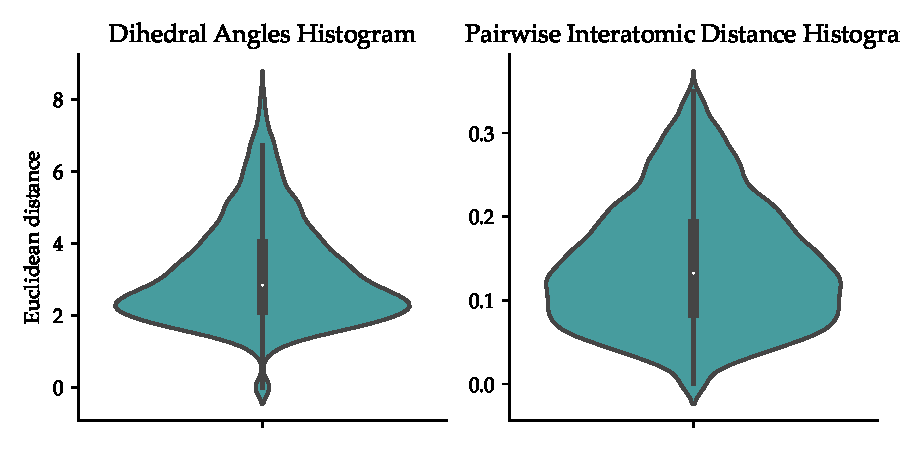
\includegraphics[width=0.6\textwidth]{./figures/results/violin_protein_descriptors.pdf}
  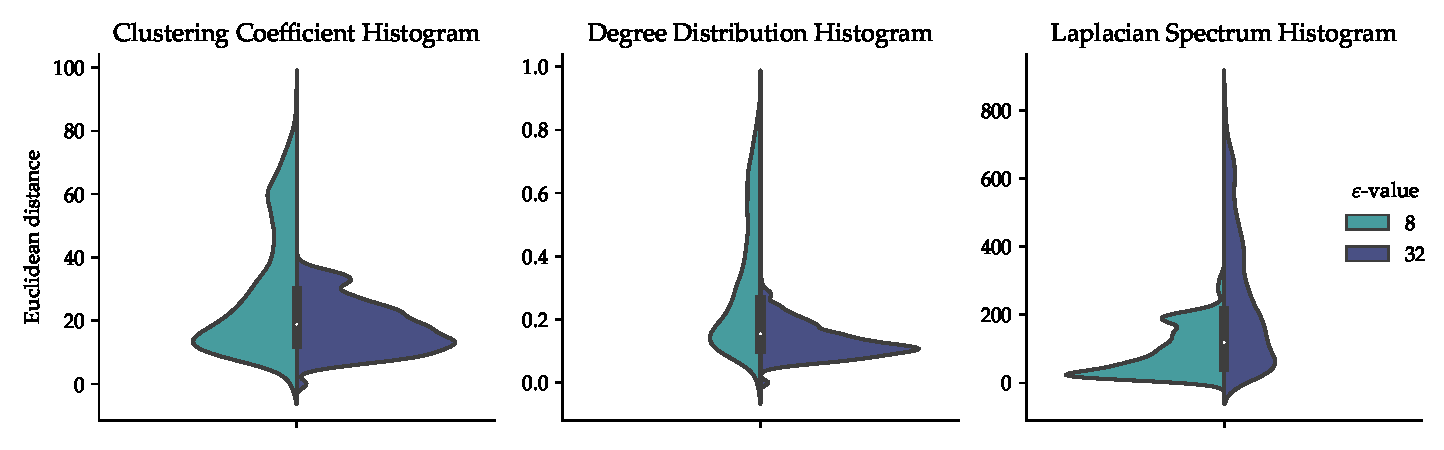
\includegraphics[width=\textwidth]{./figures/results/violin_graph_descriptors.pdf}
  \caption{Mean Euclidean distance between descriptor representations. The top
    row shows the mean distance between each of the protein descriptors
    introduced in this thesis while the bottom row shows the distance between
    each graph descriptor for two $\varepsilon$-graph extraction settings.}
\end{figure}
